V této kapitole se podíváme na skupinu semiempirických metod. Ačkoli semiempirické metody také vycházejí z řešení elektronové Schr\"{o}dingerovy rovnice, jejich rovnice obsahují dodatečné parametry, jejichž hodnoty se typicky získávají z přesnějších \textit{ab initio} výpočtů nebo se z experimentálních dat.

Semiempirické metody jsou přibližné na dvou úrovních . V první řadě, většina semiempirických metod nevychází z přesného molekulárního hamiltoniánu, ale určitého efektivního hamiltoniánu, ve kterém jsou zanedbány některé členy. Většina semiempirických metod se například soustředí pouze na valenční elektrony (příspěvek ostatních elektronů je brán jako konstanta), což celkový hamiltonián systému značně zjednoduší. 

Po určení hamiltoniánu se při odvození typické semiempirické metody postupuje obdobně jako při odvození HF rovnic. Zvolíme si konkrétní tvar vlnové funkce a zvolíme bázi (metoda MO-LCAO) a aplikací variačního principu odvodíme pracovní rovnice. V tomto kroku ale u semiempirických metod dojde k výše zmíněnému dalšímu zjednodušení. Některé členy z rovnic můžeme úplně zanedbat a položit rovno nule, anebo je můžeme považovat za parametry, se kterými dosáhneme nejlepšího souladu s experimenty pro určitý vybraný soubor molekul. Experimentálním údajem, vůči kterému se srovnáváme, mohou být termodynamické parametry daných látek. Při použití semiempirických metod je proto třeba být velmi obezřetný. Mohou fungovat skvěle pro látky, na které byla metoda parametrizována a látky jím podobné, ale pro odlišné struktury mohou hanebně selhávat.

Motivací k vývoji semiempirických metod bylo zmenšení výpočetních nároků \textit{ab initio} metod s pokud možno co nejmenším ovlivněním přesnosti. Dnes již mají vrchol své popularity za sebou. Nicméně i metody, které byly kvantitativně nepřesné, se ukázaly jako velmi užitečné, neboť dovolily kvalitativní pochopení zákonitostí chemických vazeb a jiných vlastností molekul. Na jednu takovou metodu, která nám dala známé H\"{u}ckelovo pravidlo \uv{$ 4n+2 $} pro určení aromaticity, se nyní podíváme.

\subsection{H\"{u}ckelova metoda}

H\"{u}ckelova metoda (dále jen HM) je historicky první a asi i nejjednodušší semiempirická metoda. Pro menší molekuly je pro použití této metody potřeba doslova jen tužka a papír. soustředíme se pouze na určitou skupinu elektronů, energeticky dobře oddělenou od ostatních elektronů. Typickým příkladem jsou $\pi$ vazebné elektrony v konjugovaných uhlovodících,
tedy elektrony v molekulových orbitalech složených z atomových p orbitalů.
 

Hamiltonián HM metody má tvar
\begin{equation}
H_{HMO}= \sum h_{i, eff}^\pi,
\label{rov:semiemp:ham}
\end{equation}
kde $h_{i, eff}^\pi$ je jednoelektronový potenciál $\pi$ elektronu, který v sobě obsahuje jak kinetickou energii, tak interakce s ostatními elektrony.
Z tvaru hamiltoniánu coby součtu jednoelektronových členů je zřejmé, že elektrony jsou zde považovány za nezávislé (to je zásadní rozdíl oproti metodě HF, ve které je nezávislost elektronů vyjádřena \uv{pouze} tvarem vlnové funkce). 
Konkrétní tvar těchto efektivních elektronových hamiltoniánů není specifikován, neboť, jak uvidíme dále, vlastně ani není potřeba. 

Dalším krokem je výběr báze. V případě metody HM to budou p$_z$ orbitaly všech uhlíkových atomů
\begin{equation}
\phi= \sum_i c_i \chi_i.
\label{rov:HM_MO}
\end{equation}
Matematický tvar těchto orbitalů nás ale opět nezajímá. Tím převedeme problém nalezeni vlnové funkce na jednodušší problém najití koeficientů $c_i$. Pokud tuto vlnovou funkci dosadíme do Schr\"{o}dingerovy s hamiltoniánem \eqref{rov:semiemp:ham} a aplikujeme variační princip, dostaneme soustavu sekulárních rovnic. Z podmínky pro netriviální řešení této soustavy pak platí
\begin{equation}
|\mathbb{H}-\epsilon \mathbb{S}|=0 .
\label{rov:HM_det}
\end{equation}

Pro lepší ilustraci budeme nadále uvažovat výpočet pro molekulu butadienu.
Elektronová báze se zde skládá ze čtyř p$_z$ orbitalů. Sekulární determinant zde má tvar
\begin{equation}
\begin{vmatrix}
H_{11}-\epsilon S_{11} & H_{21}-\epsilon S_{21} & H_{31}-\epsilon S_{31} & H_{41}-\epsilon S_{41}  \\
H_{12}-\epsilon S_{12} & H_{22}-\epsilon S_{22} & H_{32}-\epsilon S_{32} & H_{42}-\epsilon S_{42}  \\
H_{11}-\epsilon S_{13} & H_{23}-\epsilon S_{23} & H_{33}-\epsilon S_{33} & H_{43}-\epsilon S_{43}  \\
H_{11}-\epsilon S_{14} & H_{24}-\epsilon S_{24} & H_{34}-\epsilon S_{34} & H_{44}-\epsilon S_{44}
\end{vmatrix}
= 0 .
\end{equation}
Nyní bychom měli spočítat integrály $H_{ij}$ a $S_{ij}$, které v principu závisí na geometrii systému.
V rámci H\"{u}ckelovy aproximace na ně ale pohlížíme jako na parametry metody
a naložíme s nimi takto:
\begin{itemize}
\item zanedbáme překryvové integrály mezi AO na různých atomech tj. $S_{ij}=\delta_{ij}$;
\item integrály $H_{ii}$ položíme rovny parametru $\alpha$, těmto integrálům říkáme coulombovské integrály;
\item integrály $H_{ij}$ položíme rovno nule, pokud orbitaly nepatří sousedním atomům.
Nenulové integrály položíme rovno parametru $\beta$. Nazýváme je rezonančními integrály.
\end{itemize}

Takto zjednodušené rovnice poté vyřešíme. Nejprve najdeme vlastní čísla přes sekulární determinant a následně určíme koeficienty $c_i$. V případě butadienu bude H\"{u}ckelův sekulární determinant vypadat následovně
\begin{equation}
\begin{vmatrix}
\alpha-\epsilon & \beta & 0 & 0  \\
\beta &\alpha-\epsilon & \beta & 0  \\
0 &\beta &\alpha-\epsilon & \beta  \\
0 & 0 & \beta &\alpha-\epsilon  
\end{vmatrix}
= 0.
\end{equation}
Ve druhém kroku jsme determinant vydělili $\beta$ a zavedli substituci $x=\frac{\alpha-\beta}{\epsilon}$.
Nyní rozvojem determinantu podle prvního řádku dostaneme
\begin{equation}
x
\begin{vmatrix}
x & 1 & 0 \\
1 & x & 1 \\
0 & 1 & x \\
\end{vmatrix}
-
\begin{vmatrix}
x & 1 & 0 \\
1 & x & 1 \\
0 & 1 & x \\
\end{vmatrix}
=x^4-3x^2+1=0 \nonumber
\end{equation}
Tuto kvartickou rovnici můžeme naštěstí převést na kvadratickou pomocí substituce $y=x^2$
\begin{equation}
y^2-3y+1=0;\quad y_1=2,62;\quad y_2=0.382 \nonumber
\end{equation}
a tedy
\begin{equation}
x_{1,2}=1,62 \nonumber
x_{3,4}=0,62 \nonumber
\end{equation}
Z toho vyplývají následující hodnoty energií

$$ \epsilon_1 = \alpha+1,62\beta $$
$$ \epsilon_2 = \alpha+0,62\beta $$
$$ \epsilon_3 = \alpha-0,62\beta $$
$$ \epsilon_4 = \alpha-1,62\beta $$

Zpětným dosazením do sekulárních rovnic bychom poté dopočítali koeficienty $c_i$ a tím získali molekulové orbitaly. Ty potom obsadíme elektrony v souladu s Pauliho vylučovacím principem a celkovou energii dostaneme jako součet orbitálních energií. 
Jak nyní získáme parametry $\alpha$ a $\beta$? Vyjdeme z experimentálních dat. Parametr $\alpha$ má jednoduchou fyzikální interpretaci; jedná se o ionizační energii atomového orbitalu $p_z$, která je experimentálně známá. Důležitější je parametr $\beta$, který určuje vzájemnou separaci molekulových orbitalů. Můžeme jej získat v zásadě dvěma způsoby:
\begin{enumerate}
\item \textbf{Ze spektroskopických dat.} Parametr zvolíme tak, aby nám seděly zvolené elektronové přechody (podrobnosti viz níže). Například fitováním na molekulu naftalenu získáme hodnotu $\beta=-3,48 eV$.
\item \textbf{Z termochemických dat.} K tomu se využívá konceptu delokalizační energie dvojných vazeb. Tuto energii můžeme experimentálně naměřit například pomocí hydrogenačního tepla. Její teoretický výpočet v rámci HM si ukážeme níže. 
\end{enumerate}

Pojďme se nyní podívat na výpočet některých vlastností butadienu pomocí HM. 

\begin{figure}
\centering
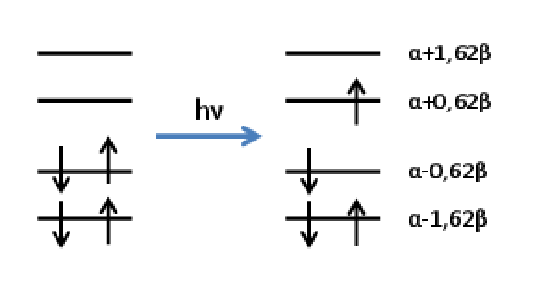
\includegraphics[scale=1]{HMbuta.eps}
\caption[Energetické hladiny butadienu]{Energetické hladiny budadienu dle H\"{u}ckelovy metody a znázonění excitovaného stavu.}
\label{obr:HMbuta}
\end{figure}

\subsubsection{Excitační energie}

Jak můžeme pomocí HM spočítat excitační energii? Formálně excitujeme jeden elektron z obsazeného do neobsazeného orbitalu (viz obrázek \ref{obr:HMbuta}) a potom spočítáme celkovou energii a od ní odečteme celkovou energii základního stavu. Pokud chceme spočítat nejnižší excitační energii butadienu, přesuneme jeden elektron z orbitalu 3 do orbitalu 2. Výsledná energie potom bude
$$
\Delta E = \epsilon_3-\epsilon_4 = 1,24 \beta = \frac{hc}{\nu} 
$$
Vlnová délka excitujícího záření vyjde 287\,nm, zatímco experimentální hodnota je kolem 200\,nm.
Soulad to není ideální, ale není ani tragický, na to že jsme jej získali tak jednoduše. HM také správně zachycuje experimentální fakt, že excitační energie se snižuje se zvyšující se délkou řetězce obsahující konjugované dvojné vazby.

\subsubsection{Delokalizační energie}

Z organické chemie si ještě možná vzpomeneme, že konjugované dvojné vazby mají jiné vlastnosti než vazby izolované.
Tuto delokalizaci můžeme vyjádřit pomocí poněkud nefyzikální veličiny \uv{delokalizační energie}.

Pokud by se dvojné vazby vzájemně neovlivňovaly, tak by mělo platit, že HM energie
\textit{n}krát-konjugovaného systému by se rovnala \textit{n}-násobku energie ethenu, který má dvojnou vazbu jen jednu. Tato rovnost ale neplatí a rozdíl je právě delokalizační energie. 

Pojďme si vše ukázat na příkladě butadienu, jehož energii již známe. Musíme tedy dopočítat energii molekuly ethenu. Pro ten vychází následující sekulární determinant. 
\begin{equation}
\begin{vmatrix}
\alpha - \epsilon & \beta \\
\beta & \alpha - \epsilon \\
\end{vmatrix}
=0
\end{equation}
z čehož
$$
(\alpha-\epsilon)^2=\beta^2
$$
$$
\alpha - \epsilon = \pm \beta
\epsilon_{1,2}= \alpha\pm \beta
$$
Pro butadien poté vychází delokalizační energie $E_D=0,472\beta=35,4 kJ/mol$.


Experimentálně můžeme míru delokalizace určit pomocí hydrogenačních tepel butadienu a ethenu.
Hydrogenační teplo ethenu (tj. entalpie reakce ethen + H$_2$ = ethan) je -136,94\,kJ/mol, zatímco hydrogenační teplo butadienu je -240\,kJ/mol. Experimentální delokalizační energie je tedy:
$$
E_D^{exp}=2\cdot139,9-240 = 33,8 kJ/mol,
$$
což je v dobrém souladu s námi vypočtenou hodnotou.

\subsubsection{Cyklické systémy a aromaticita}

Asi největším úspěchem HM bylo vysvětlení aromaticity cyklických molekul. Na obrázku \ref{obr:HMcykly} jsou znázorněny energetické hladiny cyklických systémů typu C$_n$H$_n$. Parametr $\alpha$ představuje energii elektronu v samostatném atomu uhlíku. jestliže elektron má energii nižší než  $\alpha$, interakce s okolními atomu vede k poklesu energie. Jinými slovy, dochází ke vzniku chemické vazby. energie větši než $\alpha$ indikuje destabilizaci. Pohled na diagram přitom pěkně ukazuje, odkud se vzalo známé  H\"{u}ckelovo pravidlo $4n+2$. Je totiž hned patrné, že

\begin{itemize}
\item molekuly s 4$n$+2 elektrony jsou stabilní,
\item molekuly s 4$n$+1 elektrony představují radikály,
\item molekuly s 4$n$ elektrony představují biradikály.
\end{itemize}


\begin{priklad}
\textbf{Zadání:} Jak to bude s aromaticitou cyklopropenylového radikálu? A co cyklopentadienylový radikál?

\textbf{Řešení:} V cyklopropenylu máme tři elektrony v $p_z$ orbitalech, stabilnější tedy bude cyklopropenylový kation. V cyklopentadienylu máme elektronů pět, stabilnější tedy bude cyklopendienylový anion, který se opravdu často vyskytuje jako ligand v komplexech kovů.
\end{priklad}

\begin{figure}
\centering
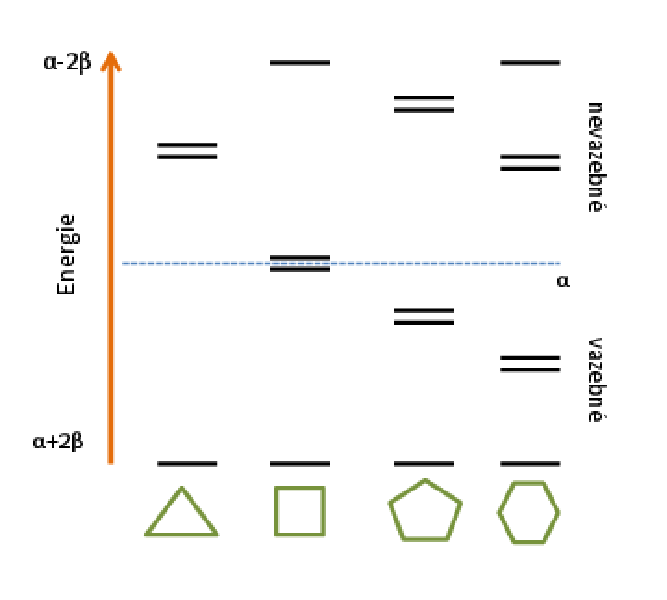
\includegraphics[scale=1]{HMcykly.eps}
\caption[Energetické hladiny cyklických uhlovodíků]{Energetické hladiny cyklických uhlovodíků obecného vzorce C$_n$H$_n$ dle H\"{u}ckelovy metody. Degenerované hladiny jsou znázorněné těsně nad sebou.}
\label{obr:HMcykly}
\end{figure}
\bigskip

%\subsubsection{Vlnová funkce z H\"uckelovy metody}


\subsection{Rozšířená H\"{u}ckelova metoda}

Hlavním vylepšením rožšířené H\"{u}ckelovy metody (RHM) je zavrhnutí $\pi$-elektronové aproximace.
Stále používáme jednoelektronový Hamiltonián a molekulové orbitaly rozvíjíme podobně jako v rovnici \eqref{rov:HM_MO}, ale zahrnujeme všechny valenční orbitaly. Atom uhlíku tedy do báze přispěje atomovými orbitaly 2s, 2p$_x$,2p$_y$ a 2p$_z$. 
Zde jsou další pravidla pro RHM:

\begin{itemize}
\item Hodnotu coulombických integrálů opět aproximujeme ionizační energií daného orbitalu.
$$H_{ii}=-I_i$$
\item Hodnoty překryvových integrálů se nezanedbávají, ale počítají se explicitně.
\item Hodnoty rezonančních integrálů se získají dle vztahu:
\begin{equation}
H_{ij}=\frac{1}{2}K(I_i+I_j)S_{ij},
\end{equation}
kde $K$ je empirická konstanta, která má obvykle hodnotu 1,75.
\end{itemize}
Opět řešíme sekulární rovnice \eqref{rov:HM_det}, ale tentokrát již matice $\mathbb{H}$ neobsahuje žádné nuly (pokud náhodou není $S_{ij}=0$ ze symetrických důvodů). Jelikož počítáme explicitně překryvové integrály, tak řešení závisí na konkrétní geometrii molekuly. Tato metoda se tedy dá použít k minimalizaci geometrie, ale výsledky často nejsou příliš kvalitní (například molekula vody vychází jako lineární).

Podobně jako v původní H\"{u}ckelově metodě tvar sekulárních rovnic nezávisí na řešení, a tudíž není třeba iterovat. Rozšířená H\"{u}ckelova metoda se proto i nyní rutinně využívá v kvantově chemických programech k prvotnímu nástřelu vlnové funkce.

\subsection{Moderní semiempirické metody}

Modernější semiempirické metody již ve svém hamiltoniánu nezanedbávají mezielektronovou repulzi.
Hamiltonián je potom téměř totožný s HF hamiltoniánem, akorát se soustředíme stále jen na valenční elektrony. Tyto metody poté iterativně řeší Roothanovy rovnice. Výpočetně nejnákladnější částí jsou stejně jako v Hartreeho-Fockově metodě dvouelektronové integrály,
\begin{equation}
\int \int \chi_i^*\chi_j\frac{1}{r_{12}}\chi_k^*\chi_l \mathrm{d}\textbf{r}_1\mathrm{d}\textbf{r}_2
\end{equation}
a proto se právě pro ně zavádí další aproximace. Velká část metod vychází z aproximace 
\begin{equation}
\phi_i(\mathbf{r}) \phi_j(\mathbf{r}) \mathrm{d}\mathbf{r} = 0 \quad i\neq j,
\label{rov:semiemp:4e}
\end{equation}
které se říká zanedbání diferenciálního překryvu. Jednotlivé semiempirické metody se liší mimo jiné tím, na které orbitaly tuto aproximaci uplatňují. Pojďme si některé přiblížit:

\begin{itemize}
\item Asi nejjednodušší metodou z této třídy je metoda \textbf{CNDO} (z angl. \textit{Complete Neglect of Differential Overlap}), která zavádí ZDO aproximaci důsledně pro všechny dvojice atomových orbitalů.

\item Méně drastickou aproximaci představuje metoda \textbf{INDO} (z angl. \textit{Intermediate Neglect of Differential Overlap}), která výše uvedený vztah neaplikuje na dvouelektronové integrály, ve kterých jsou všechny čtyři orbitaly na stejném atomu. Tato metoda byla Zernerem modifikována pro spektroskopické účely (metoda ZINDO).

Výše zmíněné metody byly vyvinuty ve skupině Johna Popla a byly parametrizovány tak, aby výsledky odpovídaly \textit{ab initio} HF výpočtům pro minimální bázi. 

\item Jiný přistup zvolil M. Dewar, který semiempirické metody začal parametrizovat tak, aby odpovídaly experimentálním hodnotám, a tím dosáhl přesnosti často větší než samotná Hartreeho-Fockova metoda. Metody AM1 (y angl. \textbf{Austin Model 1}), PM3 (z angl. \textbf{Parametric Model 3}) a jejich novější verze PM6 a PM7 jsou využívány a rozvíjeny dodnes (jejich implementace je k nalezení například ve volně dostupném programu MOPAC).

\item Kromě výše zmíněných metod existuje také hojně využívaná semiempirická metoda založená na DFT, takzvaná \textbf{DFTB} (DFT Tight Binding) a řada dalších metod, občas využívaných ke speciálním případům.

\end{itemize}
 



 
